\subsection{Sprint 5: da 2024-06-05 a 2024-06-14}
\par Durante lo \glossario{sprint} precedente, il team ha approfondito ulteriormente i framework \glossario{Flask} e \glossario{Vue.js}, che nel corso di questo sprint saranno utilizzati in sinergia per integrare \glossario{front-end} e \glossario{back-end}.
Inoltre sarà programmato un incontro con il Professore Riccardo Cardin per chiarimenti sulle tecnologie scelte. Gli obiettivi sono stati definiti in vista dell'avvicinamento dell'RTB. 

\subsubsection{Obiettivi}
\begin{itemize}
  \item Aggiornamento del \PdP\ con particolare attenzione sul preventivo a finire dello sprint 4 e la redistribuzione delle ore per ruolo;
  \item Proseguire con la stesura delle \NdP;
  \item Programmare un incontro con il Professore Riccardo Cardin per dubbi sulle tecnologie;
  \item Stesura dei verbali interni ed esterni;
  \item Ampliamento dei casi d'uso nell'\AdR\ (estensioni, errori e inserimento dei grafici dei \glossario{casi d'uso} rimanenti);
  \item Configurazione \glossario{Flask} - \glossario{Vue.js};
  \item Integrazione \glossario{back-end} e \glossario{front-end};
  \item Connessione al database con \glossario{Flask};
  \item Gestione \glossario{CRUD} dizionario dati in backend;
  \item Ultimi approfondimenti del funzionamento di txtai;
  \item Progettazione generale struttura front-end;
  \item Visualizzazione \glossario{log} e struttura del \glossario{dizionario dati} lato \glossario{front-end}.
\end{itemize}

\begin{figure}[H]
  \centering
  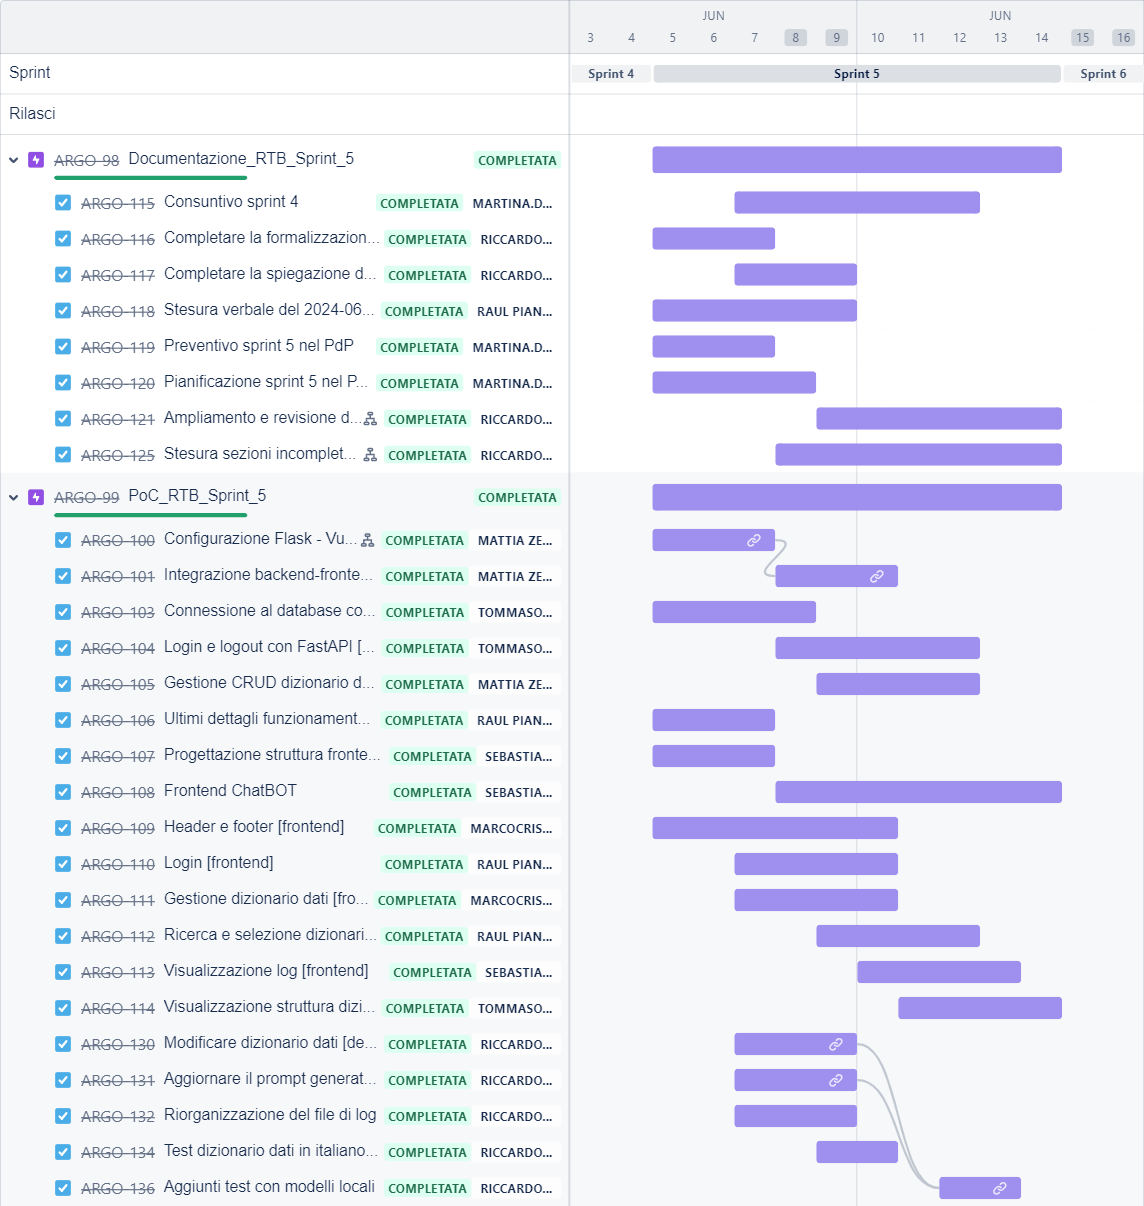
\includegraphics[width=0.90\textwidth]{assets/Pianificazione/Sprint-5/gantt.png}
  \caption{Sprint 5 - Diagramma di Gantt}\label{fig:sprint-5-gantt}
\end{figure}